%-*- coding: UTF-8 -*-
% notes.tex
%
\documentclass[UTF8]{article}
\usepackage{geometry}
\geometry{a4paper, centering, scale=0.8}
\usepackage{minted}
\usepackage{hyperref}
\usepackage{indentfirst}    % to indent the first paragraph of a section
\usepackage{graphicx}       % to insert figures
\usepackage{amsmath}        % to type some math equations
\usepackage{amssymb}        % to use some special math font
\usepackage{IEEEtrantools}  % to use IEEEeqnarray
\usepackage{algorithm2e}    % to use algorithm environment
\usepackage{multicol}       % to display some content in multi-columns
\setlength{\columnseprule}{0.4pt}   % set the rule's width of multicols
\setlength{\columnsep}{5em}         % set the sep of multicols

% Math notation
% refered to https://github.com/exacity/deeplearningbook-chinese/blob/master/math_symbol.tex
\newcommand{\Scalar}[1]{\mathit{#1}}                % Scalar, the default math font
\newcommand{\Vector}[1]{\boldsymbol{\mathit{#1}}}   % Vector
\newcommand{\Matrix}[1]{\boldsymbol{\mathit{#1}}}   % Matrix
\newcommand{\Tensor}[1]{\textsf{\textbf{#1}}}       % Tensor
\newcommand{\Set}[1]{\mathbb{#1}}                   % Set
\newcommand{\Cal}[1]{\mathcal{#1}}                  % Math Cal

% Draw the lines in a matrix, which is composed by a series of vectors
\newcommand{\vRule}{\rule{0.3pt}{10mm}}             % vertical rule
\newcommand{\hRule}{\,\rule[1mm]{10mm}{0.3pt}\,}    % horizontal rule

\title{Deep Learning Specialization \\
        Structuring Machine Learning Projects}
\author{Du Ang \\ \texttt{du2ang233@gmail.com} }
\date{\today}

\begin{document}
\maketitle

\tableofcontents
\newpage

\section{ML Strategy}
\subsection{Introduction to ML Strategy}
\subsubsection{Why ML Strategy?}
90\% is not good enough for your application, so you might try the following ideas to improve:
\begin{itemize}
    \item Collect more data
    \item Collect more diverse training set
    \item Train algorithm longer with gradient descent
    \item Try Adam instead of gradient descent
    \item Try bigger network
    \item Tray small network
    \item Try dropout
    \item Add $L_2$ regularization
    \item Network architecture
    \begin{itemize}
        \item Activation functions
        \item \# hidden units
        \item \ldots
    \end{itemize}
\end{itemize}

When trying to improve a deep learning system, you often have a lot of ideas or things you could
try, ML strategy will offer you quick and effective ways to figure out which of all of these ideas
are worth pursuing.

\subsubsection{Orthogonalization}
Orthogonalization or orthogonality is a system design property that assures that modifying an
instruction or a component of an algorithm will not create or propagate side effects to other
components of the system. It becomes easier to verify the algorithms independently from one another,
it reduces testing and development time.

When a supervised learning system is design, these are the 4 assumptions that needs to be true and
orthogonal.
\begin{enumerate}
    \item Fit training set well in cost function
    \begin{itemize}
        \item If it doesn’t fit well, the use of a bigger neural network or switching to a better
        optimization algorithm might help.
    \end{itemize}
    \item Fit development set well on cost function
    \begin{itemize}
        \item If it doesn’t fit well, regularization or using bigger training set might help.
    \end{itemize}
    \item Fit test set well on cost function
    \begin{itemize}
        \item If it doesn't fit well, the use of a bigger development set might help
    \end{itemize}
    \item Performs well in real world
    \begin{itemize}
        \item If it doesn't perform well, the development test set is not set correctly or the cost
        function is not evaluating the right thing.
    \end{itemize}
\end{enumerate}

\subsection{Setting up your goal}
\subsubsection{Single number evaluation metric}
To choose a classifier, a well-defined development set and an evaluation metric speed up the
iteration process.

\begin{figure}[htb]
    \centering
    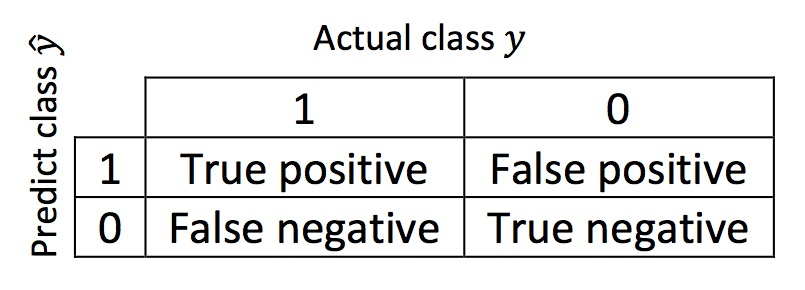
\includegraphics[width=25em]{figures/binary-confusion-matrix}
    \caption{Example: Cat vs Non-cat. $y$ = 1, cat image detected.}
\end{figure}

\paragraph{Precision}
Of all the images we predicted $y = 1$, what fraction of it have cats?

$$ \text{Precision(\%)} = \frac{Ture positive}{Number of predicted positive} \times 100
= \frac{Ture positive}{True positives + False positives} \times 100 $$

\paragraph{Recall}
Of all the images that actually have cats, what fraction of it did we correctly identifying have
cats?

$$ \text{Recall(\%)} = \frac{True positive}{Number of predicted actually positive} \times 100
= \frac{Ture positive}{True positive + False negative} \times 100 $$

The problem with using precision/recall as the evaluation metric is that you are not sure which one
is better since in this case, both of them have a good precision et recall. F1-score, a harmonic
mean, combine both precision and recall.

$$ F_1\text{ score} = \frac{2}{\frac{1}{p} + \frac{1}{r}} $$

\subsubsection{Satisficing and Optimizing metric}
There are different metrics to evaluate the performance of a classifier, they are called evaluation
matrics. They can be categorized as satisficing and optimizing matrics. It is important to note
that these evaluation matrics must be evaluated on a training set, a development set or on the
test set.

\begin{figure}[htb]
    \centering
    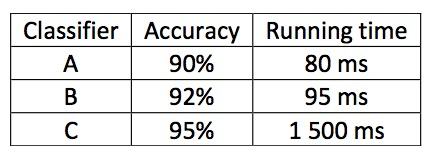
\includegraphics[width=25em]{figures/satisficing}
    \caption{Example: Cat vs Non-cat, accuracy and running time are the evaluation metrics.}
\end{figure}

Accuracy is the optimizing metric, because you want the classifier to correctly detect a cat image
as accuracy as possible. The running time which is set to be under 100ms in this example, is the
satisficing metric which mean that the metric has to meet expectation set.

The general rule is
$$ N_{\text{metric}}: \left\{\begin{array}{ll} 1 & \text{Optimizing metric} \\ N_{\text{metric}}-1
& \text{Satisficing metric} \end{array}\right. $$

\subsubsection{Train/dev/test distributions}
Setting up the training, development and test sets have a huge impact on productivity. It is
important to choose the development and test sets from the same distribution and it must be taken
randomly from all the data.

\paragraph{Guideline} Choose a development set and test set to reflect data you expect to get in
the future and consider important to do well.

\subsubsection{Size of the dev and test sets}
\paragraph{Old way of splitting data}
We had smaller dataset therefore we had to use a greater percentage of data to develop and test
ideas and models.

\begin{figure}[htb]
    \centering
    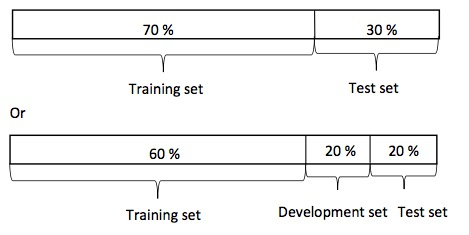
\includegraphics[width=30em]{figures/old-ways-splitting-data}
    \caption{Old ways of splitting data}
    \label{figures/old-ways-splitting-data}
\end{figure}

\paragraph{Modern era --- Big data}
Now, because a large amount of data is available, we don't have to compromised as much and can use
a greater portion to train the model.

\begin{figure}[htb]
    \centering
    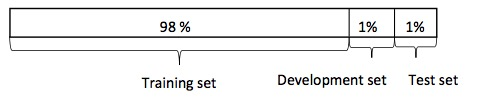
\includegraphics[width=30em]{figures/modern-era-splitting-data}
    \caption{The way of splitting data in big data era}
    \label{figures/modern-era-splitting-data}
\end{figure}

Guidelines
\begin{itemize}
    \item Set up the size of test set to give a high confidence in the overall performance of the
    system.
    \item Test set helps evaluate the performance of the final classifier which could be less 30\%
    of the whole dataset.
    \item The development set has to be big enough to evaluate different ideas.
\end{itemize}

\subsubsection{When to change dev/test sets and metrics}
\paragraph{Example: Cat vs Non-cat}
A cat classifier tries to find a great amount of cat images to show to to cat loving users. The
evaluation metric used is a classification error, as it is shown in
Figure~\ref{figures/classification-error}.

\begin{figure}[htb]
    \centering
    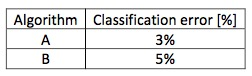
\includegraphics[width=25em]{figures/classification-error}
    \caption{The classification error of Algorithm A and Algorithm B}
    \label{figures/classification-error}
\end{figure}

It seems that Algorithm A is better than Algorithm B since there is only a 3\% error, however for
some reason, Algorithm A is letting through a lot of pornographic images.

Algorithm B has 5\% error thus it classifies fewer images but it doesn't have pornographic images.
From a company's point of view, as well as from a user acceptance point of view, Algorithm B is
actually a better algorithm. The evaluation metric fails to correctly rank order preferences
between algorithms. The evaluation metric or the development set or test set should be charged.

The misclassification error can be written as a function as follows:
$$ Error: \frac{1}{m_{dev}}\sum_{i=1}^{m_{dev}} \Cal{L}\{\hat{y}^{(i)}\neq y^{(i)}\} $$

This function counts up the nubmer of misclassified examples.

The problem with this evaluation metric is that it treats pornographic vs non-pornographic images
equally. On way to change this evaluation metrics is to add the weight term $w^{(i)}$.
$$ w^{(i)} = \left\{\begin{array}{rl} 1 & \text{if } x^{(i)} \text{ is non-pornographic} \\
10 & \text{if } x^{(i)} \text{ is pornographic} \end{array}\right. $$

The function becomes:
$$ Error: \frac{1}{\sum_w^{(i)}} \sum_{i=1}^{m_{dev}} w^{(i)} \Cal{L}\{\hat{y}^{(i)} \neq y^{(i)}
\} $$

\paragraph{Guideline}
\begin{enumerate}
    \item Define correctly an evaluation metric that helps better rank order classifiers
    \item Optimize the evaluation metric
    \item If doing well on your metric + dev/test set does not correspond to doing well on your
    application, change your metric and/or dev/test set.
\end{enumerate}

\subsection{Comparing to human-level performance}
\subsubsection{Why human-level performance?}
Today, machine learnning algorithms can compete with human-level performance since they are more
productive and more feasible in a lot of application. Also, the workflow of designing and building
a machine learning system, is much more efficient than before.

Moreover, some of the tasks that humans do are close to ``perfection'', which is why machine
learning tries to mimic human-level performance.

Figure~\ref{figures/human-level} shows the performance of humans and machine learning over time.

\begin{figure}[htb]
    \centering
    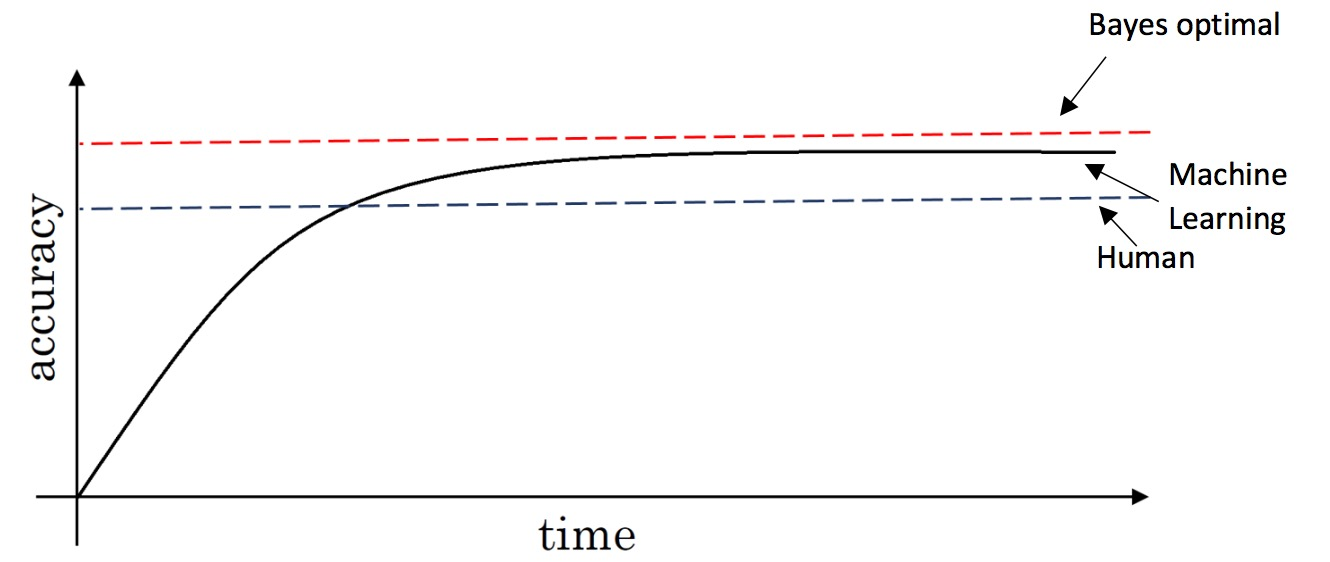
\includegraphics[width=40em]{figures/human-level}
    \caption{The performance of humans and machine learning over time.}
    \label{figures/human-level}
\end{figure}

Machine learning progresses slowly when it surpasses human-level performance. One of the reason is
that human-level performance can be close to Bayes optimal error, especially for natural perception
problem.

Bayes optimal error is defined as the best possible error. In other words, it means that any
functions mapping from $x$ to $y$ can't surpass a certain level of accuracy.

Also, when the performance of machine learning is worse than the performance of humans, you can
improve it with different tools. They are harder to use once it's surpasses human-level performance.
These tools are:
\begin{itemize}
    \item Get labeled data from humans
    \item Gain insight from manual error analysis: Why did a person get this right?
    \item Better analysis of bias/variance.
\end{itemize}

\subsubsection{Avoidable bias}
By knowing what the human-level performance is, it is possible to tell when a training set is
performing well or not.

\begin{figure}[htb]
    \centering
    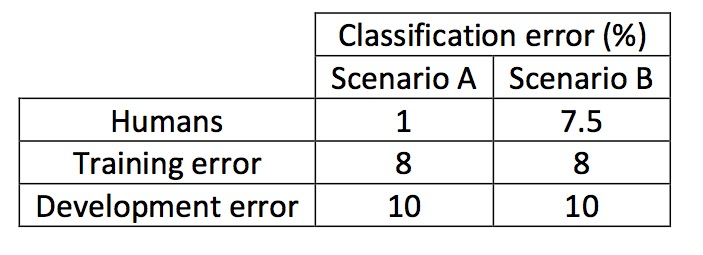
\includegraphics[width=25em]{figures/avoidable-bias}
    \caption{Different human-level in different scenarios}
    \label{figures/avoidable-bias}
\end{figure}

In the case that Figure~\ref{figures/avoidable-bias} shows, the human-level error as a proxy for
Bayes error since humans are good to identify images. If you want to improve the performance of the
training set but you can't do better than the Bayes error otherwise the training set is overfitting.
By knowing the Bayes error, it is easier to focus on whether bias or variance avoidance tactics
will improve the performance of the model.

\paragraph{Scenario A}
There is a 7\% gap between the performance of the training set and the human-level error. It means
that the algorithm isn't fitting well with the training set since the target is around 1\%. To
resolve the issue, we use bias reduction technique such as training a bigger neural networkk or
running the training set longer.

\paragraph{Scenario B}
The training set is doing good since there is only a 0.5\% difference with the human-level error.
The difference between the training set and the human-level error is called avoidable bias. The
focus here is to reduce the variance since the difference between the training set error and the
development error is 2\%. To resolve the issue, we use variance reduction technique such as
regularization or have a bigger training set.

\subsubsection{Understanding human-level performance}
Human-level error gives an estimate of Bayes error.

\paragraph{Example 1: Medical image classification}
\begin{figure}[htb]
    \centering
    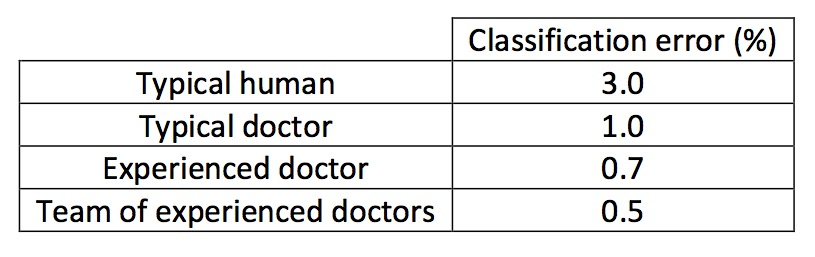
\includegraphics[width=25em]{figures/medical-image-classification}
    \caption{Medical image classification}
    \label{figures/medical-image-classification}
\end{figure}

This is an example of a medical image classification in which the input is a radiology image and
the output is a diagnosis classfication decision.

The definition of human-level error depends on the purpose of the analysis, in this case,
by definition the Bayes error is lower or equal to 0.5\%.

\paragraph{Example 2: Error analysis}

\begin{figure}[htb]
    \centering
    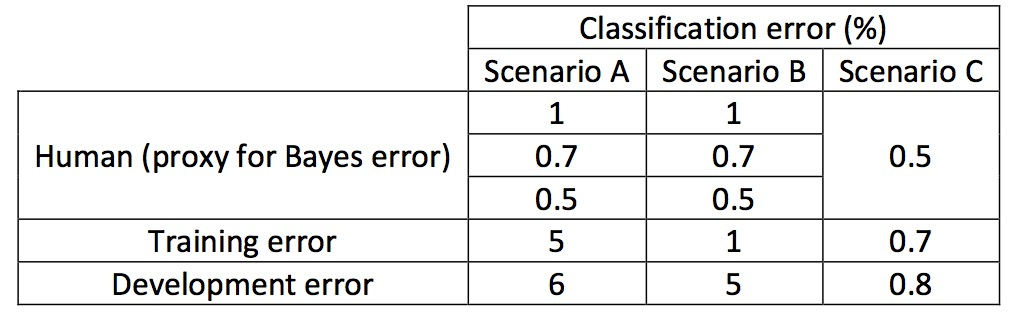
\includegraphics[width=30em]{figures/error-analysis}
    \caption{Error analysis in different scenarios according to human-levels}
    \label{figures/error-analysis}
\end{figure}

\subparagraph{Scenario A}
In this case, the choice of human-level performance doesn't have an impact. The avoidable bias is
between 4\%-4.5\% and the variance is 1\%. Therefore, the focus should be on bias reduction
technique.

\subparagraph{Scenario B}
In this case, the choice of human-level performance doesn't have an impact. The avoidable bias is
between 0\%-0.5\% and the variance is 4\%. Therefore, the focus should be on variance reduction
technique.

\subparagraph{Scenario C}
In this case, the estimate for Bayes error has to be 0.5\% since you can't go lower than the
human-level performance otherwise the training set is overfitting. Also, the avoidable bias is
0.2\% and the variance is 0.1\%. Therefore, the focus should be bias reduction technique.

\paragraph{Summary of bais/variance with human-level performance}
\begin{itemize}
    \item Human-level error --- proxy of Bayes error
    \item If the difference between human-level error and the training error is bigger than the
    difference between the training error and the development error. The focus should be on bias
    reduction technique
    \item If the difference between training error and the development error is bigger than the
    difference between the human-level error and the training error. The focus should be on
    variance reduction technique.
\end{itemize}

\subsubsection{Surpassing human-level performance}
\paragraph{Example 1: Classification task}
\begin{figure}[htb]
    \centering
    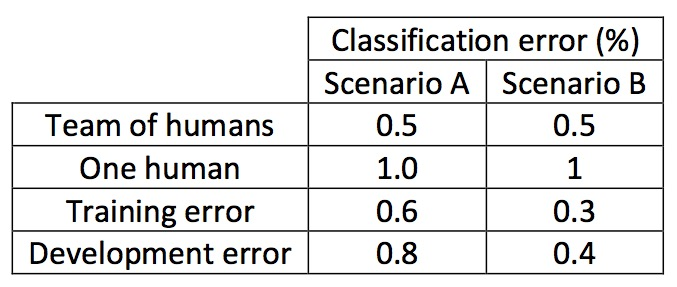
\includegraphics[width=30em]{figures/surpass-human-level}
    \caption{Classification task}
    \label{figures/surpass-human-level}
\end{figure}

\paragraph{Scenario A}
In this case, the Bayes error is 0.5\%, therefore the available bias is 0.1\% et the variance is
0.2\%.

\paragraph{Scenario B}
In this case, there is not enough information to know if bias reduction or variance reduction has
to be done on the algorithm. It doesn't mean that the model cannot be improve, it means that the
conventional ways to know if bias reduction or variance reduction are not working in this case.

There are many problems where machine learning significantly surpass human-level performance,
especially with structured data:
\begin{itemize}
    \item Online advertising
    \item Product recommendations
    \item Logistics (predicting transmit time)
    \item Loan approvals
\end{itemize}

\subsubsection{Improving your model performance}
\paragraph{The two fundamental assumptions of supervised learning}
There are 2 fundamental assumptions of supervised learning. The first one is to have a low
avoidable bias which means that the training set fits well. The second one is to have a low or
acceptable variance which means that the training set performance generalizes well to the
development set and test set. The strategy of improving your model can be seen in
Figure~\ref{figures/improve-model}.

If the different between human-level error and the training error is bigger than the difference
between the training error and the development error, the focus should be on bias reduction
technique which are training a bigger model, training longer or change the neural networks
architecture or try various hyperparameters search.

If the difference between training error and the development error is bigger than the difference
between the human-level error and the training error, the focus should be on variance reduction
technique which are bigger dataset, regularization or change the neural networks architectures or
try various hyperparameters search.

\begin{figure}[htb]
    \centering
    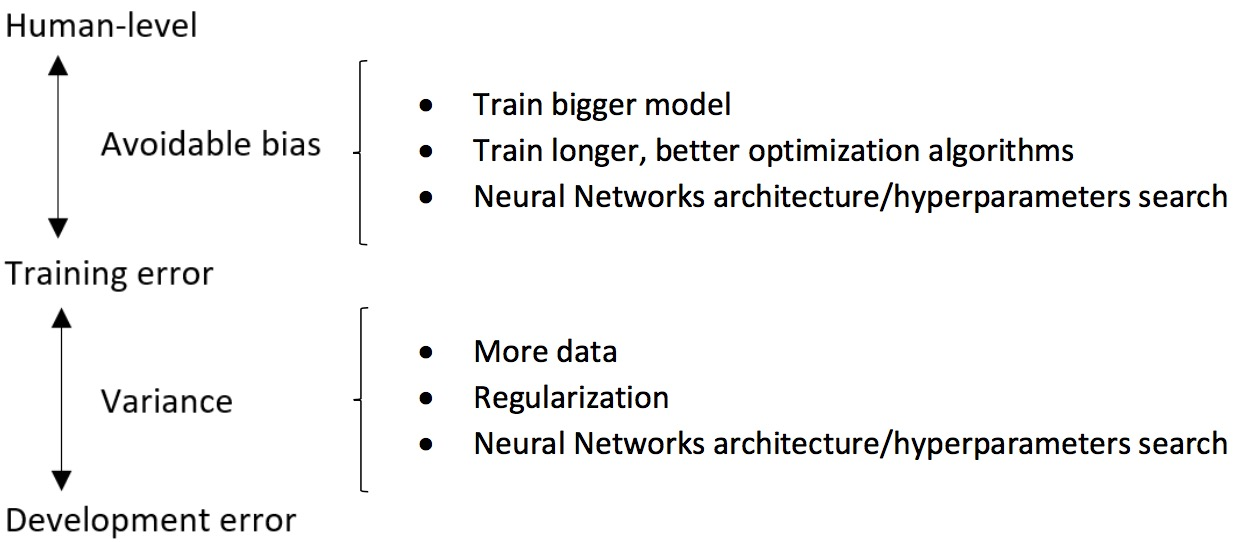
\includegraphics[width=40em]{figures/improve-model}
    \caption{The strategy to improve your models.}
    \label{figures/improve-model}
\end{figure}





















\end{document}
